\subsection{Visualización de Incertidumbre y Mapas VARISCO}
La calibración mediante CRC abre la puerta a la implementación de mapas térmicos bajo la técnica \textbf{VARISCO} (\textit{Visual Assessment of Risk Control}) \cite{segment_cp_2024}. A diferencia de los mapas de entropía tradicionales de las redes neuronales, que solo reflejan la confianza heurística del modelo y carecen de significado estadístico, los mapas VARISCO proyectan espacialmente el tamaño de los conjuntos conformes calibrados bajo diferentes niveles de riesgo $\alpha$. Al mapear la densidad de clases activas por píxel bajo una misma garantía estadística, VARISCO permite comparar de forma justa la incertidumbre epistémica entre distintas arquitecturas de redes o evaluar con fidelidad matemática qué regiones anatómicas o geográficas de la imagen presentan un riesgo real de diagnóstico erróneo.

\vspace{1em}

% =========================================================================
% ALGORITMO LISTO PARA USAR
% =========================================================================
\begin{algorithm}[H]
\caption{Calibración CRC para Segmentación Semántica Conforme}
\label{alg:crc_segmentation}
\begin{algorithmic}[1]
    \REQUIRE Conjunto de calibración $\{(X_i, Y_i)\}_{i=1, \dots n}$, modelo entrenado $\hat{f}$, nivel de error objetivo $\alpha$, cota superior de pérdida $B=1$.
    \ENSURE Parámetro óptimo de calibración $\hat{\lambda}$ y conjuntos de predicción locales para $X_{\text{test}}$.

    \STATE \textbf{Fase de Inicialización:}
    Definir una grilla de valores candidatos para el parámetro de tolerancia $\lambda \in [0,1]$.

    \STATE \textbf{Evaluación de Heurísticas:}
    Para cada imagen $i = 1, \dots, n$ en el set de calibración, extraer las probabilidades \textit{softmax} $\hat{f}(X_i)$.

    \STATE \textbf{Optimización del Umbral ($\hat{\lambda}$):}
    \FOR{cada valor candidato de $\lambda$}
        \STATE Construir los conjuntos de predicción provisionales usando el criterio LAC:
        \STATE $C_\lambda(X_i)_{ij} = \{ k \in L : \hat{f}_{ijk}(X_i) \geq 1 - \lambda \}$
        \STATE Calcular el riesgo empírico promedio mediante la pérdida por falta de cobertura:
        \STATE $\hat{R}_n(\lambda) = \frac{1}{n} \sum_{i=1}^n \left( 1 - \frac{\sum_{jk} \mathbb{I}(k \in C_\lambda(X_i)_{ij}) Y_{ijk}}{\sum_{jk} Y_{ijk}} \right)$
    \ENDFOR

    \STATE Determinar el estimador óptimo buscando el ínfimo que valida la cota superior:
    \STATE $\hat{\lambda} = \inf \left\{ \lambda : \frac{n}{n+1} \hat{R}_n(\lambda) + \frac{B}{n+1} \leq \alpha \right\}$

    \STATE \textbf{Inferencia Conforme en Test:}
    Dada una nueva imagen de prueba $X_{\text{test}}$, generar el tensor de conjuntos de predicción calibrados a nivel de píxel:
    \STATE $C_{\hat{\lambda}}(X_{\text{test}})_{ij} = \{ k \in L : \hat{f}_{ijk}(X_{\text{test}}) \geq 1 - \hat{\lambda} \}$

    \RETURN $C_{\hat{\lambda}}(X_{\text{test}})$
\end{algorithmic}
\end{algorithm}

\vspace{2em}


\begin{figure}[H]
    \centering
    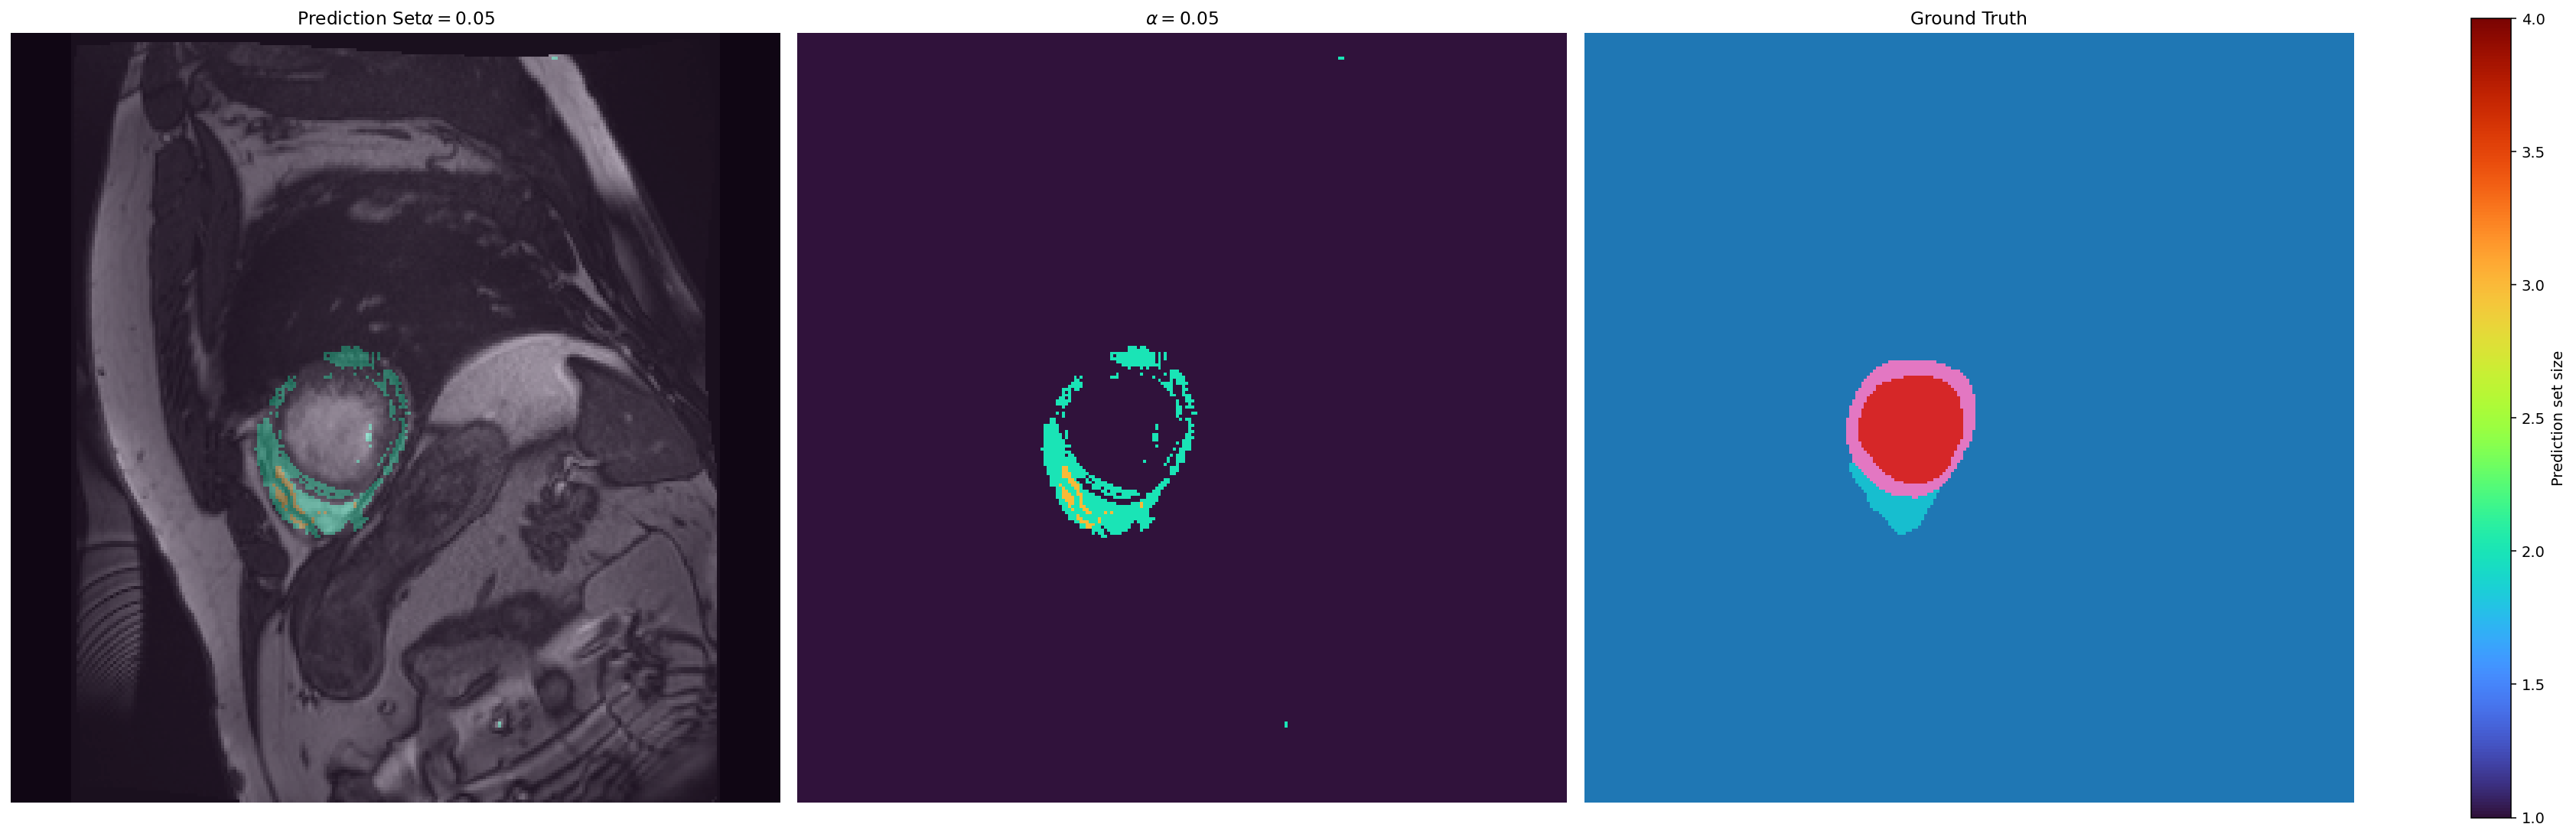
\includegraphics[width=1\linewidth]{img/prediccion_desv.png}
    \caption{Predicción, incerteza y grouth true}
    \label{fig:pred_desv}
\end{figure}

\begin{figure}[H]
    \centering
    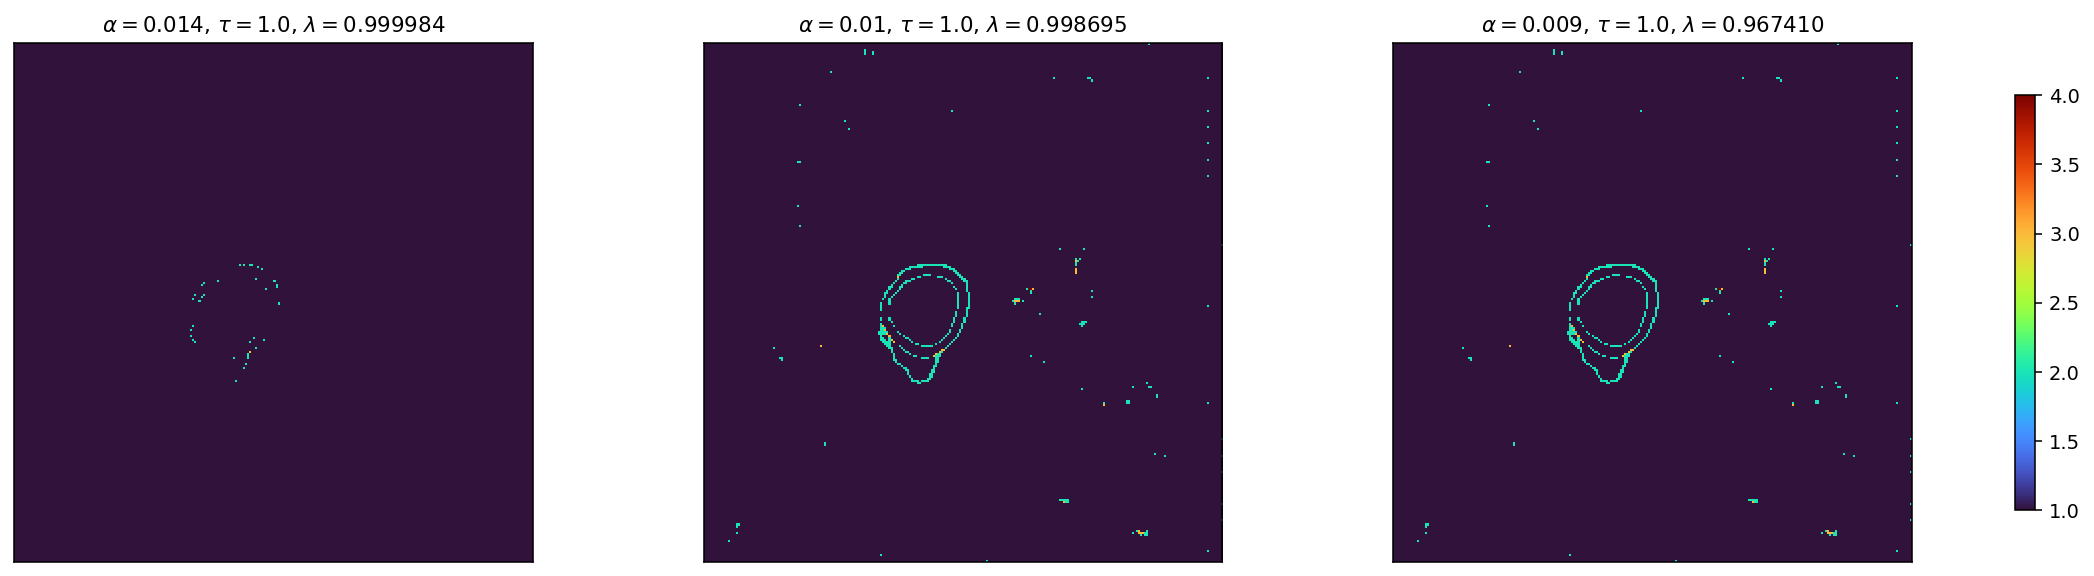
\includegraphics[width=1\linewidth]{img/variando_alphas.png}
    \caption{Incertidumbre del modelo para alphas [0.014, 0.01, 0.0090] y la temperatura $\tau = 1.0$ }
    \label{fig:desviacion_alphas}
\end{figure}

Las regiones de predicción se construyen agregando, píxel a píxel, todas las clases cuyas probabilidades predichas superen el umbral $1 - \hat{\lambda}$. Adicionalmente, se incluye de forma determinista la clase con la mayor probabilidad estimada en cada caso; esta modificación técnica previene la obtención de conjuntos vacíos en regímenes donde el umbral de aceptación resulta excesivamente estricto (valores de $\hat{\lambda}$ muy pequeños).